\documentclass{beamer}
\usetheme[subsectionpage=progressbar, background=white]{metropolis}
\usepackage[utf8]{inputenc}
\usepackage{graphicx,color}
\usepackage{amsfonts}
\usepackage{amsmath}
\usepackage{amssymb}
\usepackage{verbatim}
\usepackage{fancyhdr}
\usepackage{epigraph}
\usepackage{caption}
\usepackage{psfrag}
\usepackage{afterpage}
\usepackage[backend=biber, style=nature]{biblatex}
\addbibresource{../bibTex/thesis-library.bib}
\useinnertheme{circles}
\graphicspath{{../figures/}}
%\setbeamercovered{transparent}



\title{Nanoscale hydrodynamics near solids}
\date{June 2019}
\author{Diego Duque Zumajo}
\institute{Departamento Física Fundamental \\Universidad Nacional de Educación a Distancia}

% logo of my university
\titlegraphic{%
\begin{picture}(0,0)
\put(308,-119){\makebox(0,0)[rt]{
\includegraphics[width=1.5cm]{logo}}}
\end{picture}}

\begin{document}
\maketitle

\begin{frame}
\frametitle{Agenda}
\tableofcontents
\end{frame}

\section{Introduction}
\begin{frame}{Roadmap}
  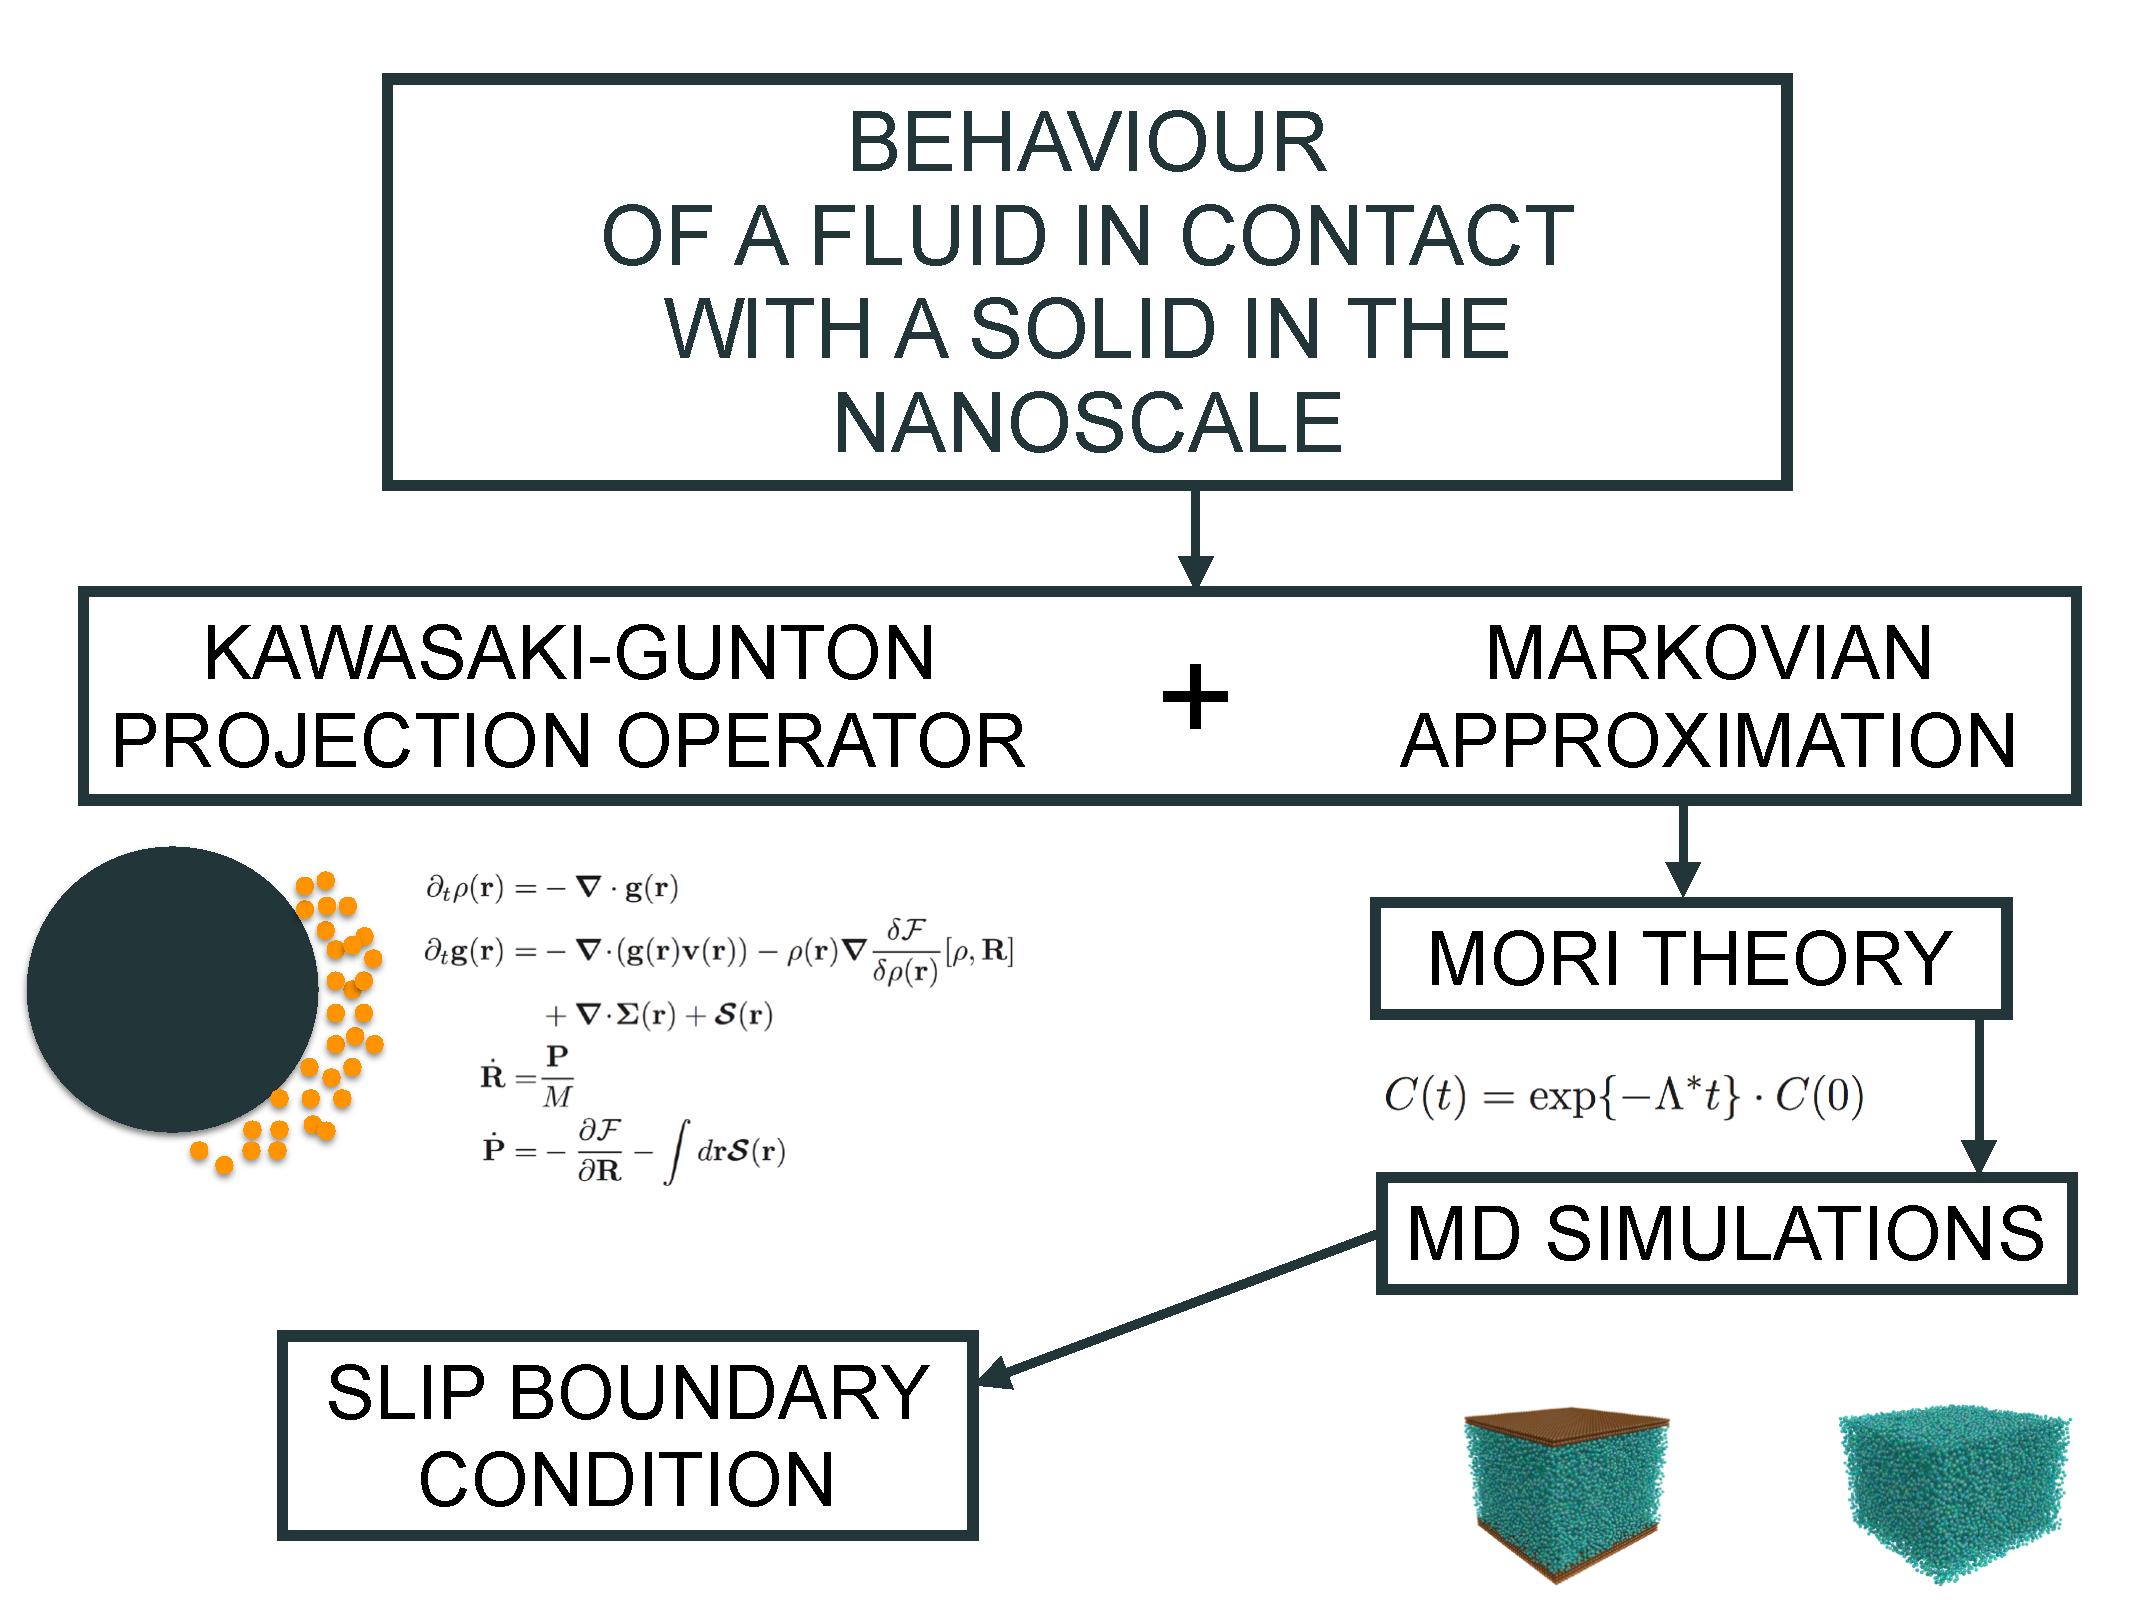
\includegraphics[width=\linewidth]{scheme-thesis}
\end{frame}
%\begin{frame}{Roadmap}
%  \begin{enumerate}
%    \item The study of \alert{the behaviour of a fluid in contact with a solid} in the nanoscale. 
%    \item Theory of Coarse-Graining in order to obtain the equations of motion of a fluid in contact with a huge solid sphere.
%    \item To address the plateau problem.
%    \item MD simulations. 
%    \item Mori theory 
%  \end{enumerate}
%\end{frame}
\begin{frame}{Derivation of the slip boundary condition}
\begin{itemize}
\item Through the  measurement of the correlation of
the  transverse  momentum  and  comparison  with  the  predictions  of
continuum  (local) hydrodynamics  \cite{Bocquet1993,Chen2015}.
\item Through
linear  response theory  relating  the  force on  the  walls with  the
velocity   of  the   fluid   \cite{Bocquet1993,Petravic2007}.
\item By formulating  linear,  in  general  non-Markovian,  conections  between
friction forces and velocities \cite{Hansen2011}, where the meaning of
this quantities is often understood implicitly.
\end{itemize}
\end{frame}

\begin{frame}{The slip problem from first principles}
  \begin{itemize}
\item Hydrodynamic equations from the microscopic dynamics of a fluid \cite{Piccirelli1968}.
\item Molecular Dynamics simulations in order to measure the transport coefficients that appear in the hydrodynamic equations in order to validate the theory.
\item The slip boundary condition is measured from a microscopic definition of the slip lenght and the position of the atomic wall. 
\end{itemize}
\end{frame}

\section{Nonequilibrium Statistical Mechanics}
\begin{frame}{The Theory of Coarse-Graining (ToCG)}
\begin{itemize}
\item The ToCG consists on eliminate the ``useless'' information about a system. 
\item Coarse grained (CG) variables.
%Selected variables with timescales much larger tha the typical molecular scales. 
\item Levels of description depending on the amount of information which one retains macroscopically.
  \begin{itemize}
    \item Macroscopic level.
    \item Microscopic level.
    \item Mesoscopic level.
    \end{itemize}
\end{itemize}
\end{frame}

\begin{frame}{The dynamics. The Kawasaki-Gunton projection operator}
  \begin{itemize}
    \item Set of CG variables $\hat{A}_i(z)$ and their conjugates variables $\lambda_i(t)$, related through the entropy $\frac{\delta S}{\delta a}=\lambda$.
    \item The aim is to derive equations of motion for the time dependent average $a_i(t)$ of the CG variables $\hat{A}_i(z)$
      \begin{align}
        a_i(t)={\rm Tr}\left[\hat{A}_i(z)\rho_t\right]
        \nonumber
      \end{align}
    \item For isolated systems with a time-independet Hamiltonian,the averages evolves according to the following equation \cite{Grabert1982}
      \begin{equation}
\frac{\partial }{\partial t} a_i(t)
= v_i(t) + \int_0^t dt' \sum_j K_{ij}(t,t') \lambda_j(t')
\nonumber
\label{ex}
\end{equation}
\end{itemize}
\end{frame}

\begin{frame}{The reversible term}
\begin{itemize}
  \item The reversible term is given by
\begin{equation}
  v_i(t) = {\rm Tr}[\overline{\rho}_t  i{\cal L} \hat{A}_i],
  \nonumber
\label{vit}
\end{equation}
where $i{\cal L}$ is the Liouville operator and $\overline{\rho}_t$ is the \alert{relevant ensemble} which maximizes the Gibbs-Jaynes entropy functional
\begin{align}
 {\cal S}[\rho]&=-{\rm Tr}\left[\rho\ln\frac{\rho}{\rho_0}\right]
\nonumber
\label{entropy}
\end{align}

\item The form of $\overline{\rho}_t$ is
\begin{equation}
\overline{\rho}(z) = \frac{1}{Z[\lambda]} \rho_0\exp\{-\lambda\!\cdot\!\hat{A}(z)\},
%\label{relens1}
\nonumber
\end{equation}
where $Z[\lambda]$ is the partition function and $\rho_0=\frac{1}{N!h^{3N}}$,   with  $h$  being   the  Planck's constant.
\end{itemize}
\end{frame}

\begin{frame}{The irreversible term}
\begin{itemize}
    \item The irreversible
      term involves the \alert{memory kernel}
\begin{equation}
K_{ij}(t,t') =
{\rm Tr}\left[\overline{\rho}_{t'} 
  \left({\cal Q}_{t'} i{\cal L}\hat{A}_j\right) G_{t't}
\left({\cal Q}_{t } i{\cal L}\hat{A}_i\right)\right],
\nonumber
\label{ker}
\end{equation}
where   the  Kawasaki-Gunton   projection  operator   ${\cal  Q}_{t'}$
applied  to an  arbitrary  function
$\hat{F}(z)$ is
\begin{align}
  {\cal Q}_{t'}\hat{F}(z) &= \hat{F}(z)- {\rm Tr}[\overline{\rho}_{t'} \hat{F}]
%\nonumber\\
-\sum_i(\hat{A}_i(z)-a_i(t'))\frac{\partial }{\partial a_i(t')}
{\rm Tr}[\overline{\rho}_{t'} \hat{F}]
\label{Q}
\nonumber
\end{align}

\item The time ordered projected propagator $G_{t't}$ is given by
\begin{align}
  G_{t't}&=1
+\sum_{n=1}^\infty \int_{t'}^tdt_1\cdots\int_{t'}^{t_{n-1}}dt_n
i{\cal L}{\cal Q}_{t_n}\cdots  i{\cal L}{\cal Q}_{t_1}
\nonumber\\
&\equiv T_+\exp\left\{\int_{t'}^t dt''  i{\cal L}{\cal Q}_{t''}\right\},
\nonumber
\end{align}
where $T_+$ ensures that the operators are ordered from left to right as time increases.
\end{itemize}
  
\end{frame}

\begin{frame}{Markovian equation. Kawasaki-Gunton projection operator}
  \begin{itemize}
     \item Whenever a clear separation of timescales exists between the evolution of the averages and the decay of the memory kernel can be approximate by the memory-less equation
\begin{equation}
  \frac{\partial}{\partial t}a_i(t) = v_i(t) + \sum_j D_{ij}(t) \lambda_j(t)
\label{ex2}
\nonumber
\end{equation}
\item The  dissipative matrix  is  given  by  the Green-Kubo  formula
\begin{equation}
D_{ij}(t)=\int_0^{\Delta t} dt'\left\langle 
{\cal Q}_t i{\cal L}\hat{A}_j\exp\{i{\cal L}t'\}{\cal Q}_t i{\cal L}\hat{A}_i
\right\rangle^{\lambda(t)}
\label{dij}
\nonumber
\end{equation}
\end{itemize}
\end{frame}

\begin{frame}{The dynamics. Mori theory}

\end{frame}



\end{document}
